
\section{ Static Nonlinearities: Complex Cells}
\label{sec: StaticNonlinearitiesForComplexCells}

\begin{rem}
  % While linear methods, such as spike-triggered averages, are useful for revealing the properties of simple cells, at least to a first approximation, complex cells display features that are fundamentally incompatible with a linear description.
  The spatial receptive fields of complex cells cannot be divided into separate ON and OFF regions that sum linearly to generate the response. Areas where light and dark images excite the neuron overlap, making it difficult to measure and interpret spike-triggered average stimuli.
\end{rem}

\begin{prin}
  \label{prin:complexCellSpatialResponse}
  Like simple cells, complex cells are \emph{selective to the spatial frequency and orientation} of a grating. However, unlike simple cells, complex cells respond to bars of light or dark no matter where they are placed within the overall receptive field. Likewise, the responses of complex cells to grating stimuli show \emph{little dependence on spatial phase}.
\end{prin}

\begin{defn}
  The phenomenon that a complex cell is selective for a particular type of image independent of its exact spatial position within the receptive field is called the \emph{spatial-phase invariance}.
\end{defn}

\begin{rem}
  The spatial-phase invariance of complex cells may represent an early stage in the visual processing that ultimately leads to position-invariant object recognition.
\end{rem}

\begin{rem}
  Complex cells also have temporal response characteristics that distinguish them from simple cells.
\end{rem}

\begin{prin}
  \label{prin:complexCellTemporalResponse}
  Complex cell responses to moving gratings are approximately constant, not oscillatory as in examples \ref{exm:explain2} and \ref{exm:directionSensitivity}. The firing rate of a complex cell responding to a counterphase grating oscil lating with frequency $\omega$ has both a constant component and an oscillatory component with a frequency of $2\omega$, a phenomenon known as \emph{frequency doubling}.
\end{prin}

\begin{rem}
  To give a first approximation to complex-cell responses, the key
  observation comes from Equation \ref{equ:2.34}, which shows how the linear response estimate of a simple cell depends on spatial phase for an optimally oriented grating with $K$ not too small.
\end{rem}

\begin{prop}
  Consider two such responses, labeled $L_1$ and $L_2$, with preferred spatial phases $\phi$ and $\phi-\pi/2$. Including both the spatial and the temporal response factors, we find, for preferred spatial phase $\phi$
  \begin{equation}
    \label{equ:2.39}
    L_1=AB(\omega,K)\cos(\phi-\Phi)\cos(\omega t-\delta),
  \end{equation}
  where $B(\omega, K)$ is a temporal and spatial frequency-dependent amplitude factor. For preferred spatial phase $\phi-\pi/2$,
  \begin{equation}
    \label{equ:2.40}
    L_2=AB(\omega,K)\sin(\phi-\Phi)\cos(\omega t-\delta).
  \end{equation}
  Thus we have,
  \begin{equation}
    \label{equ:2.41}
    L_1^2+L_2^2=A^2B^2(\omega,K)\cos^2(\omega t-\delta).
  \end{equation}
\end{prop}
\begin{proof}
  Equation \ref{equ:2.39} follows from Equation \ref{equ:2.34}, Equation \ref{equ:2.40} follows from $\cos(\phi-\pi/2-\Phi) = \sin(\phi-\Phi)$ and Equation \ref{equ:2.41} follows from $\cos^2(\phi-\Phi)+\sin^2(\phi-\Phi) = 1$.
\end{proof}

\begin{coro}
  \label{coro:spatialPhaseInvariantResponse}
  We can describe the spatial-phase-invariant response of a complex cell by writing
  \begin{equation}
    \label{equ:2.42}
    r(t)=r_0+G(L_1^2+L_2^2),
  \end{equation}
  for some constant $G$. 
\end{coro}

\begin{exm}
  \label{exm:selectivityOfComplexCell}
  Selectivity of the complex cell model (Equation \ref{equ:2.42}) in response to a sinusoidal grating is shown in the following figures.
  The width and preferred spatial frequency of the Gabor functions underlying the estimated firing rate satisfy $k\sigma = 2$.
  \begin{center}
    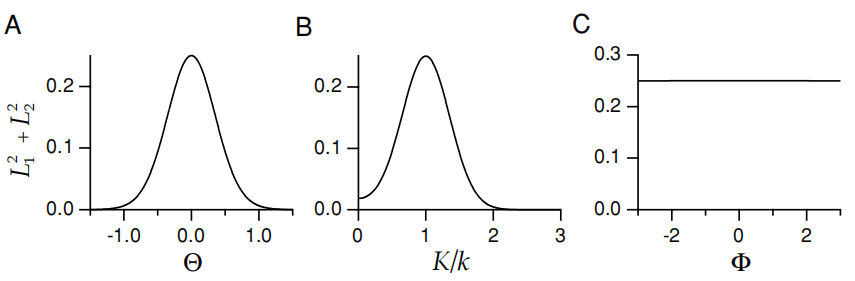
\includegraphics[scale=0.3]{./png/spatialPhaseInvariantExm1}
  \end{center}
  \begin{enumerate}[A]
  \item The complex cell response estimate, $L_1^2+L_2^2$, as a function of stimulus orientation $\Theta$ for a grating with the preferred spatial frequency $K = k$.
  \item $L_1^2+L_2^2$ as a function of the ratio of the stimulus spatial frequency to its preferred value, $K/k$, for a grating oriented in the preferred direction $\Theta = 0$.
  \item $L_1^2+L_2^2$ as a function of stimulus spatial phase $\Phi$ for a grating with the preferred spatial frequency and orientation, $K = k$ and $\Theta = 0$.
  \end{enumerate}
\end{exm}

\begin{rem}
  The response of the model complex cell is tuned to orientation and spatial frequency, but the spatial phase dependence, illustrated for a simple cell in figure C of Example \ref{exm:selectivityOfComplexCell}, is absent. In computing the curve for figure C in Example \ref{exm:selectivityOfComplexCell}, we used the exact expressions for $L_1$ and $L_2$ from the integrals in equations \ref{equ:2.31} and \ref{equ:2.32}, not the approximation used in Equation \ref{equ:2.34} to simplify the previous discussion. Although it is not visible in the figure, there is a weak dependence on $\Phi$ when the exact expressions are used.
\end{rem}

\begin{prop}
  The complex cell response given by equations \ref{equ:2.41} and \ref{equ:2.42} reproduces the frequency-doubling effect seen in complex cell responses.
\end{prop}
\begin{proof}
  This follows from the identity
  \begin{equation}
    \label{equ:2.43}
    \cos^2(\omega t-\delta)=\frac{1}{2}\cos(2(\omega t-\delta))+\frac{1}{2},
  \end{equation}
  where the last term on the right side of this equation generates the
constant component of the complex cell response to a counterphase grating.
\end{proof}

\begin{exm}
  Temporal responses of model simple and complex cells to a counterphase grating is shown in the following figures.
  \begin{enumerate}[(A)]
  \item The stimulus $s(x, y,t)$ at a given point $(x, y)$ plotted as a function of time.
  \item The rectified linear response estimate of a model simple cell to this grating with a temporal kernel given by Equation \ref{equ:2.29} with $\alpha$ =  1/(15 ms).
  \item The ``frequency-doubled'' response of a model complex cell with the same temporal kernel but with the estimated rate given by a squaring operation rather than rectification. The background firing rate is $r_0$ = 5 Hz.
  \end{enumerate}
  Note the temporal phase shift of both B and C relative to A.
  \label{exm:compareSimpleComplex}
  \begin{center}
    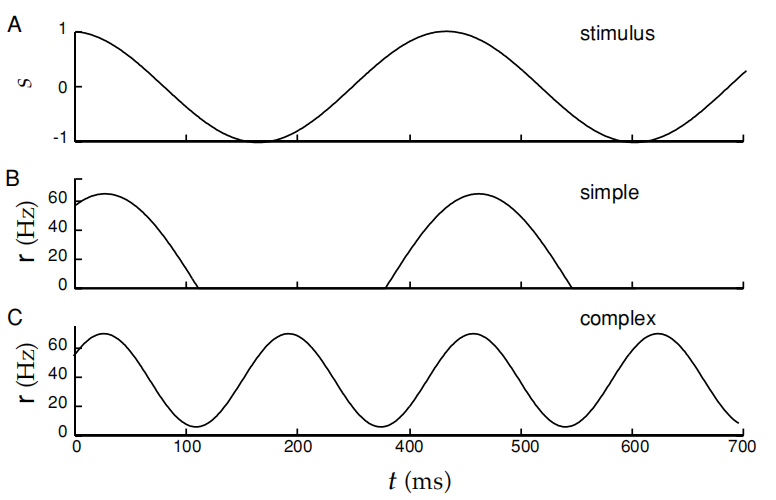
\includegraphics[scale=0.32]{./png/compareSimpleComplex}
  \end{center}
\end{exm}

\begin{defn}
  \label{def:energyModel}
  The description of a complex cell response that we have presented is called an \emph{energy model} because of its resemblance to the equation for the energy of a simple harmonic oscillator. The pair of linear filters used, with preferred spatial phases separated by $\pi/2$, is called a \emph{quadrature pair}.
\end{defn}

\begin{prop}
  We can write the complex cell response as the sum of the squares of four rectified simple cell responses,
  \begin{equation}
    \label{equ:2.44}
    r(t)=r_0+G([L_1]_+^2+[L_2]_+^2+[L_3]_+^2+[L_4]_+^2),
  \end{equation}
  where the different $[L]_+$ terms represent the responses of simple cells with preferred spatial phases $\phi$, $\phi+\pi/2$, $\phi+\pi$, and $\phi+3\pi/2$.
\end{prop}
\begin{proof}
  Because of rectification, the terms $L_1^2$ and $L_2^2$ cannot be constructed by squaring the outputs of single simple cells. However, they can each be constructed by summing the squares of rectified outputs from two simple cells with preferred spatial phases separated by $\pi$.
\end{proof}

\begin{rem}
   While such a construction is possible, it should not be interpreted too literally because complex cells receive input from many sources, including the LGN and other complex cells. Rather, this model should be viewed as purely descriptive. Simple mechanistic models of complex cells are described at the end of this chapter.
\end{rem}




 





%%% Local Variables:
%%% mode: latex
%%% TeX-master: "../notesOnFluidMechanics"
%%% End:
